\documentclass{article}
\usepackage[utf8]{inputenc}

\usepackage{natbib}
\usepackage{graphicx}
\usepackage{fancyhdr}
\pagestyle{fancy}

\begin{document}
\pagenumbering{Roman}
\begin{titlepage}
   \begin{center}
        Kalamazoo College\\
        Senior Individualized Project in Computer Science
       \vspace*{3cm}
 
       \textbf{SQL query generation from a decorator declared GraphQL schema}
 
       \vspace{0.5cm}
        Thesis Subtitle
 
       \vspace{1.5cm}
 
       \textbf{Joshua Gibson}
 
       \vspace{4cm}
 
       Faculty Supervisor:\\
       Dr. Eric Barth\\
       Assistant Provost and Professor of Mathematics\\
       Kalamazoo College\\
       Kalamazoo, MI
       
       \vspace{3cm}
       
       A paper submitted in partial fulfillment of the requirements for the degree of Bachelor of Arts at Kalamazoo College
 
   \end{center}
\end{titlepage}


\section{Introduction}
There is a theory which states that if ever anyone discovers exactly what the Universe is for and why it is here, it will instantly disappear and be replaced by something even more bizarre and inexplicable.
There is another theory which states that this has already happened.

\begin{figure}[h!]
\centering
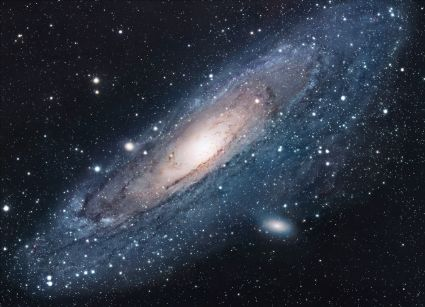
\includegraphics[scale=1.7]{universe}
\caption{The Universe}
\label{fig:universe}
\end{figure}

\section{Conclusion}
``I always thought something was fundamentally wrong with the universe'' \citep{adams1995hitchhiker}

\bibliographystyle{plain}
\bibliography{references}
\end{document}
